% !TeX root = ../main.tex
% Add the above to each chapter to make compiling the PDF easier in some editors.

\chapter{Literature Review}\label{chapter:literature}
The literature review sheds light on the understanding of deepfakes, their history,
the technology driving them, the publicly available tools that create them, and
the ethical, legal, and societal issues they raise. Additionally, it examines the
countermeasures that have been developed to detect and deter them.

\section{Techniques Used in Deepfakes}\label{chapter:techniques}
Deepfakes are underpinned by significant advancements in artificial intelligence (\ac{AI})
and machine learning (ML), particularly the areas of deep learning and neural
networks. Central to the creation of deepfakes are two techniques:
autoencoders and \ac{GAN}.

\subsection{Autoencoders}
Autoencoders, are a type of neural network used for learning
efficient encodings or representations of input data~\cite{doi:10.1126/science.1127647}.
In 2006, Hinton et al.~\cite{10.1145/3297156.3297210,doi:10.1126/science.1127647}
raised the concept of deep learning. This idea quickly gained significant attention,
making deep learning a primary focus of research worldwide~\cite{simonyan2015deep}.
The structure of autoencoders has two main parts: an encoder, which simplifies an
image into a latent space\footnote{Latent space is a compressed representation of data where essential
	features are captured in lower dimensions~\cite{enwiki:1169655673}}~\cite{latent-space-medium}, and a decoder,
which rebuilds the image using that simplified representation~\cite{latent-space-medium,enwiki:1170192786}. Deepfakes use this
setup with a common encoder that translates a person into this latent space. This simplified
representation captures essential details about their face and body stance. This can subsequently
be decoded using a model specifically trained for the intended target. So, in other words,
during the encoding phase, it extracts facial details from two distinct individuals,
identifying and storing the shared facial characteristics. Subsequently, in the decoding phase,
it presents the information of these two individuals. The encoding of one person can be
swapped with another, enabling the face of one person to be superimposed onto another
in an eerily realistic manner.

\begin{figure}[ht]
	\centering
	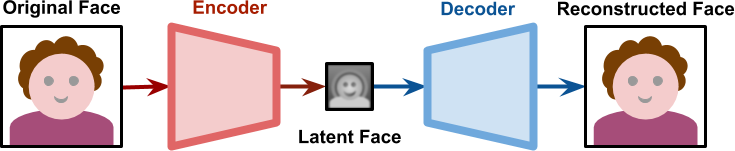
\includegraphics[scale=0.45]{figures/deepfakes_00d}
	\caption{Autoencoders common structure. Figure from~\cite{autoencoders-image-alazucconi}}\label{fig:autoencoders}
\end{figure}

The figure in~\autoref{fig:autoencoders} presents an image going
into an encoder. The outcome is a simplfied version of that face, ofeten called a latent face~\cite{autoencoders-image-alazucconi}.
Depending on the setup, this latent face might not resemble a typical face. However, when it goes
through a decoder, it's turned back into a face.

An example of using autoencoders is Fakeapp, developed by a Reddit user for deepfake generation~\cite{s22124556,fakeapp-app}.
The process requires encoding and decoding pairs to interchange faces between input and
output images. Distinct image datasets train each pair, but the encoder parameters remain
consistent across both networks. Consequently, both encoder pairs utilize the same network. Given
the consistent facial features such as the eyes, nose, and mouth across various images,
this method allows the encoder to easily recognize similarities between two sets of facial images.

\subsection{Generative Adversarial Networks}
In the field of \ac{AI} and \ac{ML}, two primary methods exist: supervised and unsupervised learning.
The former relies on labeled data\footnote{In machine learning, data labeling involves attaching
	meaningful tags to raw data so that models can learn from it~\cite{labeled-data}.}
for predictions, whereas the latter does not. Noteably, each method has its distinct advantages and
nuances~\cite{ibm-machine-learning}.

\textit{Supervised learning} is a machine learning approach which uses labeled datasets to
instruct algorithms in data categorization or predict outcomes. By using labeled inputs and outputs,
the model calculates its precision and refines itself over time~\cite{supervised-unsupervised}.
Supervised learning can be categorized into two data mining tasks: classification and regression.
Classification involves accurately sorting data into specific groups, like distinguishing between
newspapers and magazines. Meanwhile, regression uses algorithms to discern the relationship between
dependent and independent variables~\cite{ibm-machine-learning}.

\textit{Unsupervised learning} applies algorithms to group and analyze unlabeled datasets,
identifying hidden patterns without requiring human guidance~\cite{supervised-unsupervised}.

Among the concepts and techniques used in \ac{ML}, discriminative and generative models stand out
as two widely used approaches~\cite{generative-discriminative}. So a \textit{generative model}
assesses the distribution of a dataset to determine the probability of a specific example. On the
contrary, a \textit{discriminative model} predicts unseen data using conditional probability
and is applicable for both classification and regression tasks~\cite{generative-discriminative2}.

There are two main types of generative models, \ac{GAN}s and \ac{VAE}~\cite{generative-discriminative}. \ac{GAN}s
introduced by Goodfellow et al.~\cite{goodfellow2014generative}, envolve two
competing neural networks: a generator and a discriminator. The generator produces
fake samples and the discriminator distinguishes between the real and fake samples.
Within a given training dataset, this method is adept at producing new data that mirrors the
statistical properties of the training data. For instance, when taught using pictures, a \ac{GAN}
can create new images that look very real and similar to the original pictures~\cite{enwiki:1169846514}.
While \ac{GAN}s were initially introduced as generative models for unsupervised learning,
they have demonstrated utility in semi-supervised~\cite{salimans2016improved},
fully supervised~\cite{pix2pix2017}, and reinforcement learning~\cite{ho2016generative} contexts.

At the heart of \ac{GAN}s lies the principle of `indirect' training via the discriminator.
This iterative process improves the quality of the generated samples over time as
the generator learns to create more realistic fakes to fool the discriminator. This
arms race pushes the boundaries of what \ac{GAN}s can create, contributing to the
production of deepfakes that are increasingly difficult to detect~\cite{brock2019large}.

\textbf{\ac{GAN}s with alternative architectures.} Various variants of \ac{GAN} structures
and associated generative models exits. In the original paper~\cite{goodfellow2014generative},
\ac{GAN}s were designed using \ac{MLP} and \ac{CNN}. Later on, many other generative models and
architectures, as described in~\autoref{tab:gans}, were introduced~\cite{gans-versions}.

\begin{table}[htpb]
	\caption{Some of \ac{GAN}s with alternate architectures~\cite{gans-versions,enwiki:1169846514}}\label{tab:gans}
	\centering
	\small
	\begin{tabularx}{\textwidth}{l X}
		\toprule
		\textbf{Types of \ac{GAN}s}    & \textbf{Description}                                                \\
		\midrule
		Conditional GAN (CGAN)         & If both the generator and discriminator of
		\ac{GAN}s are conditioned on supplementary information, y, the model becomes
		conditional. This additional data, y, might be class labels or data from
		different sources. To condition the model, y is inputted
		into both the discriminator and generator as an extra input
		layer~\cite{mirza2014conditional}.                                                                   \\
		\addlinespace
		Dual GAN (DGAN)                & A version of \ac{GAN}, named DualGAN,
		uses two networks trained concurrently using two sets of unlabeled images.
		One network is designed for image generation, while the other distinguishes
		between generated and actual images. DualGAN effectively learns two image translators,
		making it suitable for diverse image-to-image translation activities~\cite{yi2018dualgan}.           \\
		\addlinespace
		Stack GAN (StackGAN)           & A modified version of \ac{GAN} uses multiple generators
		stacked together to create a more lifelike image. Stacked \ac{GAN}s compose a
		network designed to produce high-quality images~\cite{zhang2017stackgan}.                            \\
		\addlinespace
		Cycle GAN (CycleGAN)           & CycleGAN is a method for automatically converting
		images from one domain to another, without the need for paired data samples~\cite{zhu2020unpaired}.  \\
		\addlinespace
		Superresolution GAN (SRGAN)    & A \ac{GAN} designed to transform low-resolution images into
		high-resolution outputs. Super-resolution \ac{GAN}s use a combination of deep networks
		and adversarial networks to enhance the clarity of the input data~\cite{ledig2017photorealistic}.    \\
		\addlinespace
		Deep convolutional GAN (DCGAN) & A \ac{GAN} that employs deep convolutional networks
		for both the generator and discriminator. This \ac{GAN} relies solely on convolution
		and deconvolution layers. Studies suggest that images produced by the DCGAN
		architecture exhibit notably reduced noise~\cite{radford2016unsupervised}.                           \\
		\addlinespace
		Self-attention GAN (SAGAN)     & The SAGAN facilitates attention-based, extended-range
		dependency modeling in image creation. In SAGAN, cues from all feature areas can
		be utilized to produce details. Additionally, the discriminator ensures that intricate
		details in separate parts of the image are consistent with each other~\cite{zhang2019selfattention}. \\
		\bottomrule
	\end{tabularx}
\end{table}

\subsection{Variational Autoencoders}
Recent developments have seen the rise of \ac{VAE} and their use in deepfake
generation~\cite{kingma2022autoencoding}. Unlike traditional autoencoders, \ac{VAE}s introduce
a probabilistic spin to the encoding and decoding processes. The encoder, often
designed using neural networks like the feedforward convolutional network,
learns to encode input data into a latent space. The decoder, also based
on a convolutional neural network, then reconstructs the original input
from this latent space~\cite{vae-gan}. This allows for the
generation of new faces by sampling from the learned distribution, enhancing the
ability of the deepfake technology to generate entirely new, but convincing, faces.

While both \ac{VAE}s and \ac{GAN}s are used for image generation, their methodologies differ.
One primary distinction is their training approach. \ac{VAE}s use an unsupervised learning
technique, aiming to maximize the likelihood of the generated output relative to the
input and compress the input into a latent space. Conversely, \ac{GAN}s are trained
in a supervised learning technique, striving for equilibrium between the generator
and discriminator, where the former seeks to fool the latter. Furthermore, \ac{VAE}s
often have a more straightforward training process compared to \ac{GAN}s because they
don't require tight coordination between their components. Additionally, due to their
advanced capabilities, \ac{GAN}s are often used for demanding tasks such as
super-resolution and image-to-image translation. On the other hand, \ac{VAE}s are
predominantly used for image denoising and generation~\cite{vae-gan}.

\section{Publicly Available Deepfake Generation Tools}\label{chapter:publicly}
As deepfake technology has evolved, so too has the ease of access to this technology.
There are now several deepfake generation tools that are freely available and relatively
easy to use, drastically lowering the bar for entry into the world of deepfakes.

\subsection{DeepFaceLab}\label{sec:deepfacelab}
DeepFaceLab\footnote{\url{https://github.com/iperov/DeepFaceLab}}~\cite{perov2021deepfacelab,10.1117/12.2631297}
was developed to address the challenges and inefficiencies typically
observed in deepfake generation models~\cite{s22124556}. This refined framework,
facilitates face-swapping~\cite{perov2021deepfacelab}. The architecture incorporates
an `encoder' and `destination decoder', separated by an `inter' layer, and
concludes with an `alignment' layer. To extract features, it uses the 2DFAN~\cite{Bulat_2017}
heat map-based facial landmark algorithm, and for face segmentation,
it utilizes the TernausNet~\cite{iglovikov2018ternausnet}.

\begin{figure}[htpb]
	\centering
	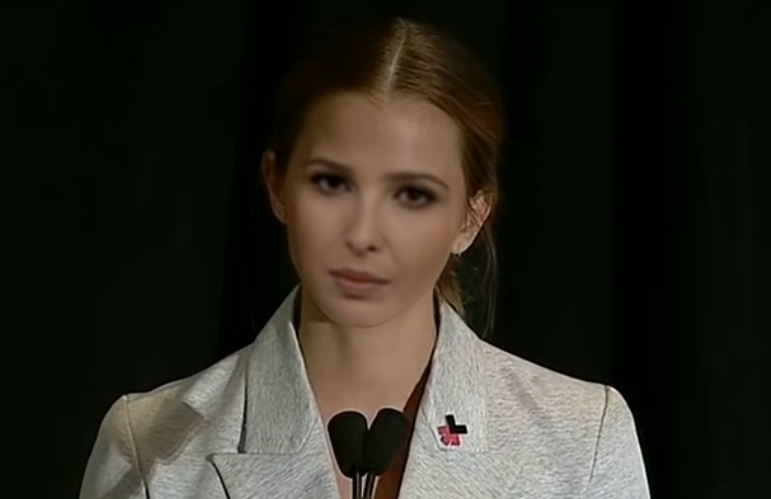
\includegraphics[scale=0.36]{figures/ivanka-deepfacelab}
	\caption{Deepfake of Ivanka Trump impersonating Emma Watson. Screenshot
		from our own generated deepfake video dataset with DeepFaceLab.}
\end{figure}

Known for offering greater functionality and control over the deepfake creation
process, DeepFaceLab has been used in several high-profile deepfake videos.
Its sophisticated technology combines the power of \ac{GAN}s and autoencoders,
leading to highly realistic face swaps in videos. DeepFaceLab offers tools
for every step of the deepfake creation process, including face extraction,
training, and video creation. This comprehensive suite of tools, combined
with its high-quality results, make it a popular choice among deepfake creators.

\subsection{FaceSwap}\label{sec:faceswap}
Faceswap typically refers to the replacement of one person's face with another's
in images or videos. In this context, it signifies a specific technique
implemented in~\cite{faceswap}. The method operates frame-by-frame for both
source and target videos until one ends. Within each image, distinct
facial landmarks such as face contour, eyes, mouth, and other distinguishing
facial features are identified. Utilizing the landmarks from the source image,
a 3D representation of the source actor's face is constructed. This is then
adjusted to align with the target actor's facial landmarks and integrated
into the target image. After processing each frame, the result is a video
wherein the target actor's face is substituted by the source
actor's~\cite{deepfakes-thesis,9897972,Korshunova_2017_ICCV}.

\begin{figure}[htpb]
	\centering
	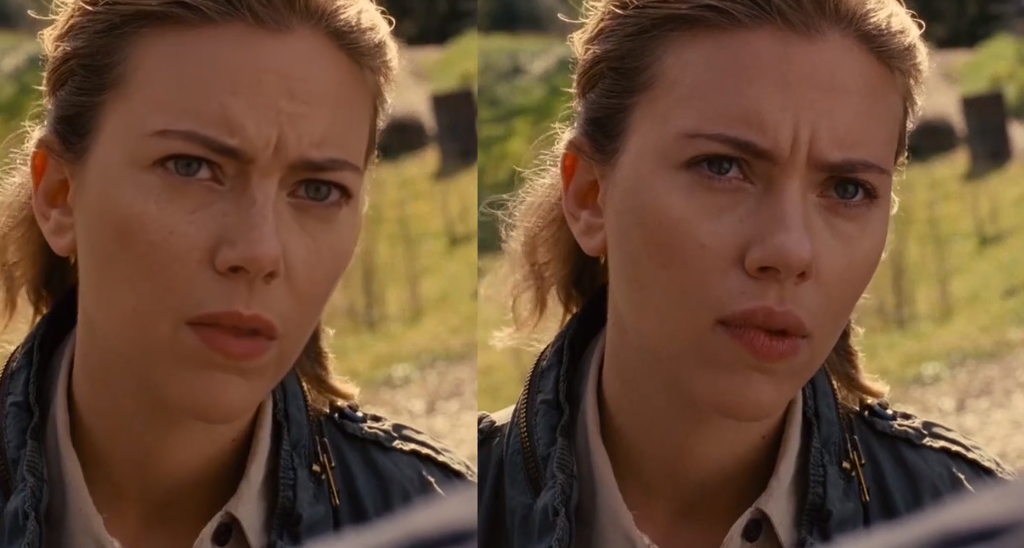
\includegraphics[scale=0.32]{figures/emma-stone-faceswap}
	\caption{Deepfake of Emma Stone impersonating Scarlett Johansson using
		Faceswap. Screenshot from~\cite{emma-stone-faceswap}.}
\end{figure}

This community-based deepfake tool stands out with its open-source nature,
providing the user with a choice of multiple \ac{AI} models. It caters to
varying levels of experience and computing resources, making it accessible
to a wide range of users. Besides its technical merits,
FaceSwap\footnote{\url{https://faceswap.dev}} emphasizes the ethical use
of deepfake technology, warning against non-consensual use of a person's
likeness. It is more than just a tool; it's a community where people can
learn, discuss, and share knowledge about deepfakes.

\subsection{Stable Diffuison}\label{sec:stable-diffusion}
Recently, image synthesis methods using diffusion models centered on denoising
techniques~\cite{ho2020denoising} have gained popularity because of their impressive
outcomes in generating artificial artwork~\cite{10.1145/3588015.3589842}.
Notably, latent diffusion models like \ac{SD}~\cite{rombach2022highresolution}
empower individuals to produce images from textual prompts effectively,
even using personal computers.

Introduced in 2022~\cite{rombach2022highresolution}, Stable Diffusion is a deep learning
model utilizing diffusion methods, primarily for generating intricate images based
on textual inputs. It also has applications in inpainting\footnote{Inpainting refers
	to the restoration technique where absent or damaged sections of an artwork are
	replenished to display a complete image~\cite{enwiki:1164523541}.},
outpainting, and facilitating image-to-image conversions guided by a text
prompt~\cite{sd-hugging-face}. The model was a collaborative effort from the CompVis Group
at Ludwig Maximilian University of Munich~\cite{enwiki:1169859793}, Runway,
Stability AI\footnote{\url{https://stability.ai/stablediffusion}}, and
several non-profit organizations~\cite{sifted-2020,sd-lmu,stabilityai}.

As a latent diffusion model, Stable Diffusion is a type of deep generative neural network.
Its code and model parameters are publicly available~\cite{sd-github}, and it's
compatible with consumer-grade hardware having a GPU with a minimum of
8 GB~\cite{enwiki:1169859793}. This is in contrast to previous models like DALL-E~\cite{dall-e}
and Midjourney~\cite{midjourney}, which were restricted to cloud-based access~\cite{enwiki:1169859793,sd-theverge}.

\begin{figure}[htpb]
	\centering
	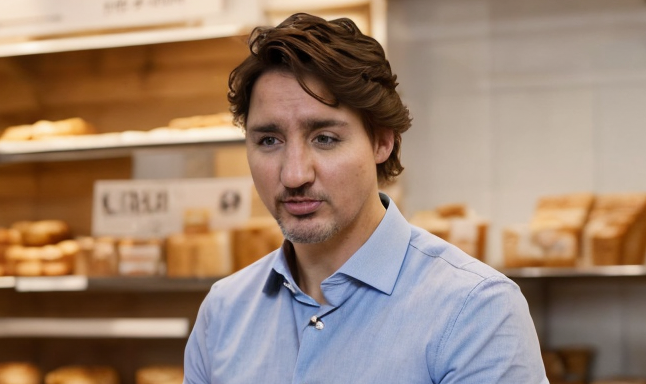
\includegraphics[width=0.59\columnwidth]{figures/justion-trudeau-stable-diff}
	\caption{Deepfake of Justin Trudeau created with Stable Diffusion.
		Screenshot from our own generated deepfake video dataset with Stable Diffuison.}
\end{figure}

Stable Diffusion models utilize a diffusion process to generate realistic synthetic
images from a simple Gaussian noise, achieving impressive results in the generation of
deepfake images~\cite{wu2022unifying}. One of the benefits of diffusion models
is that they can capture complex, multi-modal distributions in a way that
other generative models may struggle with. This makes them particularly
well-suited for tasks like deepfake generation, where capturing the
detailed, multi-modal distribution of human faces is essential.

\subsection{Neural Textures}
Introduced by Thies et al.~\cite{thies2019deferred}, Neural Textures represent
a method for the storage, transmission, and rendering of learned
neural representations in the context of computer graphics.
By rendering with learned features instead of geometric detail, Neural
Textures allow for more efficient representations, enabling high-quality,
photorealistic image synthesis and editing. Specifically, in the realm of
deepfakes, Neural Textures, as shown in~\autoref{fig:neural_textures}, can be trained to synthesize person-specific
details, resulting in high-quality face swaps or manipulation of facial
expressions in videos.

\begin{figure}[htpb]
	\centering
	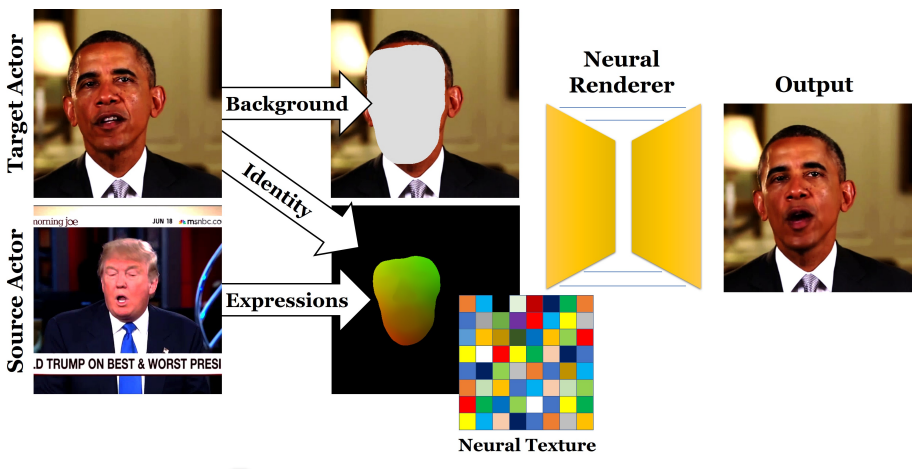
\includegraphics[scale=0.55]{figures/neural_textures}
	\caption{The reenactment synthesis process uses expression transfer
		to generate a UV map of the target actor that reflects the source
		actor's expression. This map, along with a background image, is
		processed by a neural renderer to create the final reenactment.
		Expression alteration is achieved by training a unique neural
		texture and renderer for the target actor, resulting in a
		manipulated video as shown in the image from~\cite{thies2019deferred}.}\label{fig:neural_textures}
\end{figure}

Neural textures utilize a UV-map\footnote{UV mapping involves projecting a 3D model's surface
	onto a 2D plane for the purpose of texture mapping~\cite{enwiki:1169139226}.}
connecting elements in the texture map to object points, allowing the creation of a
viewpoint-specific texture. Integrating this into a trained deferred neural renderer
produces an image from the designated viewpoint, as illustrated in~\autoref{fig:neural-textures2}.
While neural textures have various uses, Thies et al.~\cite{thies2019deferred} highlight
facial video manipulation. \autoref{fig:neural_textures} demonstrates this application,
paralleling the Face2Face~\cite{thies2020face2face} method. Training videos establish a
3D face model of the target actor. Additionally, a unique neural texture and deferred neural
renderer are crafted for this actor. Leveraging the Face2Face expression transfer
technique, a UV-map from the target video is adjusted to mirror the source actor's
expressions. With this UV-map, the neural texture, and renderer, the manipulated video emerges.

\begin{figure}[htpb]
	\centering
	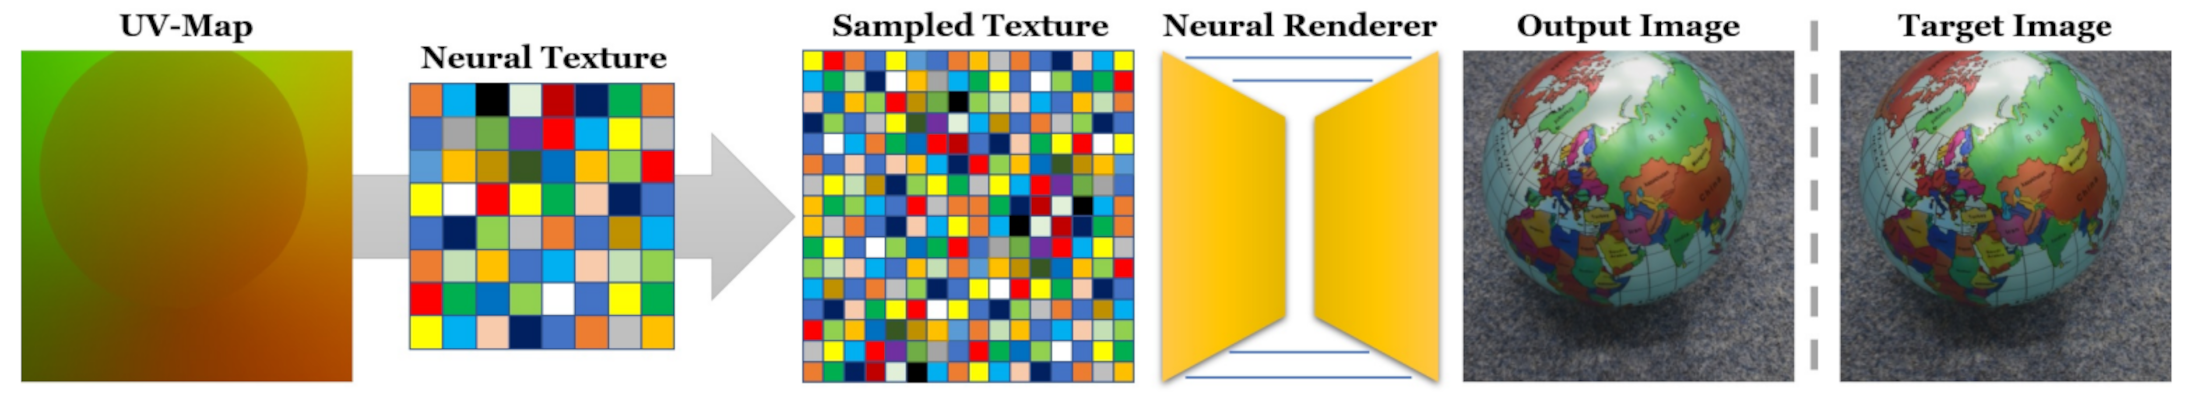
\includegraphics[scale=0.25]{figures/neural_textures2}
	\caption{Overview of neural rendering pipeline~\cite{thies2019deferred}.}\label{fig:neural-textures2}
\end{figure}

\subsection{FaceApp}\label{sec:faceapp}
While not a deepfake tool in the traditional sense,
FaceApp\footnote{\url{https://www.faceapp.com/}} has gained popularity due
to its ability to transform photos of faces in various ways, such as aging,
de-aging, gender swapping, and adding smiles~\cite{wirth2023interface}.
Introduced in 2017~\cite{wirth2023interface} by the Russian startup Wireless Lab, now known
as FaceApp Technology Limited, the FaceApp software enables users to undertake
detailed photo and video modifications. These include aging or rejuvenating facial
appearances, merging two faces, incorporating intricate facial expressions like smiles,
and utilizing the debated `gender swap' function.

\begin{figure}[htpb]
	\centering
	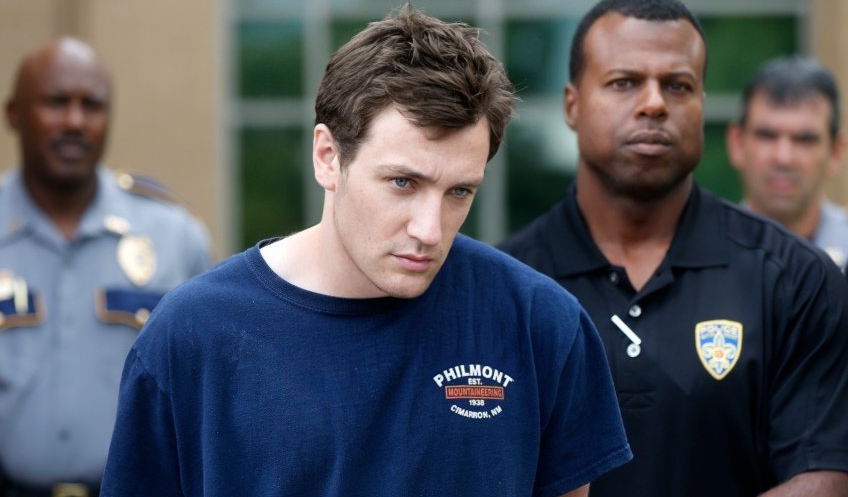
\includegraphics[width=0.61\columnwidth]{figures/faceapp}
	\caption{Deepfake created with FaceApp. Screenshot from our own generated deepfake image
		dataset with FaceApp.}
\end{figure}

The tool leverages neural network technology for its transformations, leading to surprisingly
realistic results that have significantly contributed to the broader conversation
around the manipulation of digital imagery~\cite{faceapp}. FaceApp has
been both praised for its technological achievements and criticized for
its potential privacy and consent issues~\cite{warzel2019faceapp}, reflecting the wider debates
surrounding the ethical implications of deepfake technology.

In essence, FaceApp's image processing capabilities go beyond just simple pixel-altering
image filters. Initially, each image is transformed into a multi-dimensional vector which
might subsequently serve as a foundation for modification --- essentially a reshuffling
of the neural weights in the network~\cite{faceapp-article1}. When using FaceApp's tools,
the \ac{CNN} superimposes specific features onto the chosen portrait or selfie, features
that have been extracted from its training dataset. Thanks to sophisticated image recognition
techniques, precise automatic feature adjustments are made, resulting in notably photorealistic
effects. Intriguingly, while fundamentally transforming the image, FaceApp preserves
unique facial features~\cite{faceapp-medium}. This allows users to perceive alterations, like aging or
rejuvenation, as authentic modifications to their own faces~\cite{wirth2023interface,faceapp-article2}.

\section{Ethical and Legal Concerns}\label{chapter:legal}
The rise of deepfakes has brought with it a number of ethical and legal concerns.
At the forefront is the issue of consent, as deepfakes often involve the
use of a person's identity without their permission. This has been
particularly common in the creation of deepfake pornography, leading
to significant harm and distress for the individuals involved~\cite{chesney2019deep}.

There are also concerns about the potential misuse of deepfakes in spreading
disinformation and propaganda. Deepfakes could be used to manipulate public
opinion, interfere in elections, or even incite violence~\cite{deepfakes-business-insider,partnershiponai}.
The realistic nature of deepfakes makes it difficult for the average viewer
to distinguish truth from fake, further exacerbating these risks.

In journalism, the rise of deepfakes presents both a significant
challenge and an ethical dilemma. Journalists must not only cope with
the complex task of verifying the authenticity of deepfake content
but also think about the ethical implications of using \ac{AI}-generated
content in their reporting. Misuse of deepfakes could lead to the spread of
false information, shaking people's faith in the media~\cite{doi:10.1177/2056305120903408}.

Furthermore, the use of deepfake technology can be used to fabricate evidence in
legal cases, potentially leading to miscarriages of justice. As deepfakes become
increasingly indistinguishable from real videos, the legal system will need to
find ways to authenticate digital evidence and mitigate the risk of deepfake-generated
evidence~\cite{chesney2019deep}.

The business sector is not immune to the impact of deepfakes either. Businesses
could fall victim to deepfake scams, in which \ac{AI}-generated audio or video
is used to impersonate a company employee or other authority figure.
These scams could lead to significant financial losses or damage to a
company's reputation~\cite{MUSTAK2023113368}.

Lastly, in deepfake detection, a crucial concern is the issue of
false positives and negatives. A false positive, where a real video is wrongly
flagged as a deepfake, could have serious consequences, such as the unnecessary
spread of panic or unwarranted damage to an individual's reputation. On the
other hand, a false negative, where a deepfake is not detected and is thus
taken as genuine, can lead to the propagation of disinformation or fraud.
These challenges underscore the need for highly careful deepfake detection methods~\cite{roessler2019faceforensicspp}.

\section{Existing Countermeasures and Detection Methods}\label{chapter:countermeasures}
The rise of deepfakes demand effective countermeasures and detection methods
to ensure information integrity and maintain public trust
in digital content. As deepfake generation techniques have become more advanced,
detection approaches have adapted accordingly. Many of these
approaches use machine learning, particularly deep learning techniques,
leveraging similar technologies that power deepfakes to combat them.

The general idea of deepfake detection is based on identifying inconsistencies
or anomalies that typically arise during the process of creating deepfakes. These
can be artifacts left by the specific algorithm used, unusual patterns in the
distribution of the pixel values, or unnatural physical characteristics
such as inconsistent lighting or improper blinking patterns~\cite{Agarwal_2019_CVPR_Workshops}.

One approach to detect deepfakes is frequency-based analysis, where the focus is
on the differences in frequency patterns between original and deepfaked videos.
These methods, like the one proposed by Durall et al.~\cite{durall2020unmasking},
take advantage of the fact that, deepfake generation algorithms usually function in
spatial domain~\cite{spatial-domain}. As a result, they may produce distinct inconsistencies
within the frequency domain.

Another widely used approach is the \ac{CNN} based detection. This type of deep
learning model has shown excellent performance in various image and video
processing tasks due to its ability to learn hierarchical patterns in the data.
For deepfake detection, \ac{CNN}s can be trained to learn the differences between
real and fake images or videos, thus distinguishing deepfakes from the original
media~\cite{nguyen2018capsuleforensics}.

Another promising approach is the use of autoencoders for deepfake detection.
Autoencoders are a type of neural network that are trained to reconstruct
their input data. By training an autoencoder on a large amount of real face
data, it can learn to recreate real faces very well, but struggle to recreate
deepfakes, allowing the detection of deepfakes based on the reconstruction
error~\cite{cozzolino2017recasting}.

Recent advancements have led to the development of deepfake detection techniques
that analyze physiological signals. For instance, Li et al.~\cite{li2018ictu}
developed a method based on the observation that real videos contain physiological
signals that are driven by blood flow, such as heart rate. These signals, they
found, are not well preserved in synthetically generated data and thus provide
a new cue for deepfake detection.

It's important to note, however, that as deepfake generation techniques
continue to evolve, the effectiveness of these detection methods can diminish.
The constant race between deepfake creation and detection presents ongoing
challenges for researchers and developers in maintaining the efficacy of these
countermeasures.